\section*{\fontsize{16}{14}\selectfont Aim: Getting familiar with function oriented design tools for making dataflow diagrams.}

\section*{DFD}
A data flow diagram (DFD) is a graphical representation of the "flow" of data through an information system, modelling its process aspects. A DFD is often used as a preliminary step to create an overview of the system, which can later be elaborated. DFDs can also be used for
the visualization of data processing (structured design).\\
A DFD shows what kind of information will be input to and output from the system, where the data will come from and go to, and where the data will be stored. It does not show information about the timing of process or information about whether processes will operate in sequence or in parallel.\\\\
Data flow diagrams are also known as bubble charts. DFD is a designing tool used in the top-down approach to Systems Design. This context-level DFD is next "exploded", to produce a Level 1 DFD that shows some of the detail of the system being modeled. The Level 1 DFD
shows how the system is divided into sub-systems (processes), each of which deals with one or more of the data flows to or from an external agent, and which together provide all of the functionality of the system as a whole. It also identifies internal data stores that must be present in order for the system to do its job, and shows the flow of data between the various parts of the system.\\\\
Data flow diagrams are one of the three essential perspectives of the structured-systems analysis and design method SSADM. The sponsor of a project and the end users will need to be briefed and consulted throughout all stages of a system's evolution. With a data flow diagram, users are able to visualize how the system will operate, what the system will accomplish, and how the system will be implemented. The old system's dataflow diagrams can be drawn up and compared with the new system's data flow diagrams to draw comparisons to implement a more efficient sy
stem. \\\\
Data flow diagrams can be used to provide the end user with a physical idea of where the data they input ultimately has an effect upon the structure of the whole system from order to dispatch to report. How any system is developed can be determined through a data flow diagram model.\\
In the course of developing a set of levelled data flow diagrams the analyst/designer is forced to address how the system may be decomposed into component sub-systems, and to identify the transaction data in the data model.
\begin{figure}[!th]
\centering
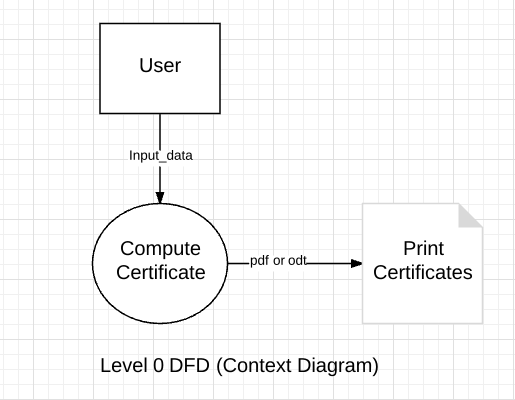
\includegraphics[width=0.7\linewidth]{input/images/dfd0.png}
\caption{Level 0}
\label{fig:image1}
\end{figure}

\begin{figure}[!th]
\centering
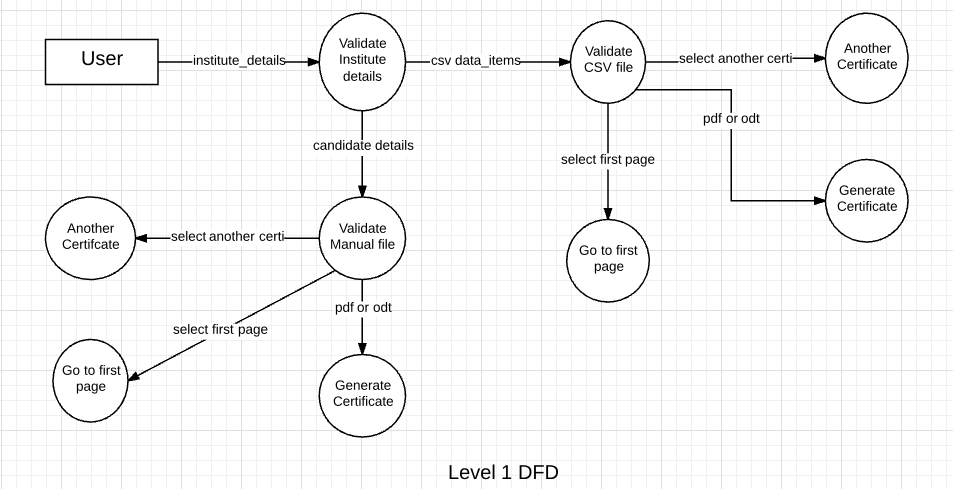
\includegraphics[width=0.7\linewidth]{input/images/dfd_1.png}
\caption{Level 1}
\label{fig:image1}
\end{figure}

\begin{figure}[!th]
\centering
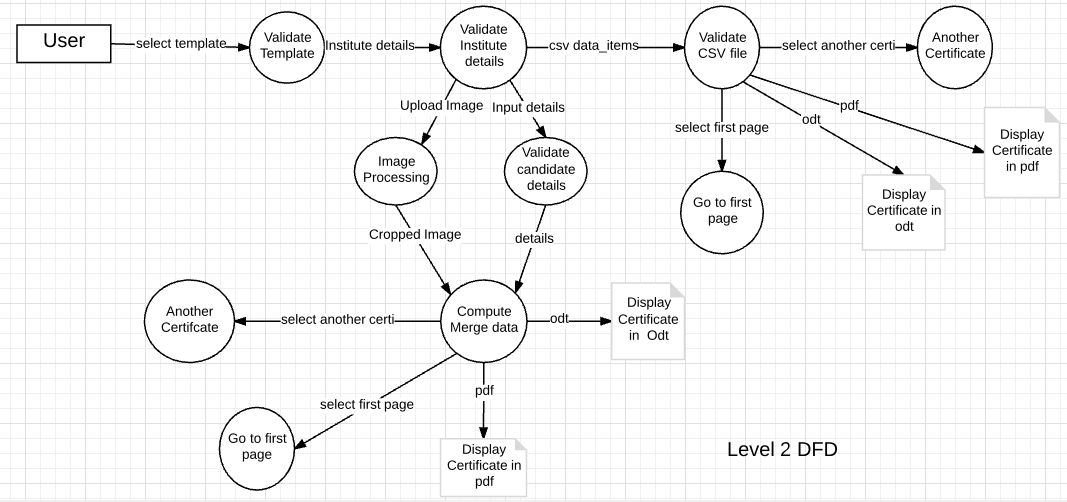
\includegraphics[width=0.7\linewidth]{input/images/dfd_2.png}
\caption{Level 2}
\label{fig:image1}
\end{figure}
\section*{Data Dictionary}
input\_data: institution\_details, select template, csv data\_items, candidate details\\
institution details: Institution name, Aided Status, Insitution tagline, Affiliation, Event, Topic, Signature, Designation\\
csv data\_items: csv file + tar file of images\\
First name: string\\
Institution name: string\\
image: upload image, crop image\\
output: certificate in pdf or odt\\
pdf: file format\\
odt: file format\\
Another Certificate: period /* another certifiate with same institution details*/\\
Go to first page: period /mave to home page */\\



 

